\documentclass[12pt,a4paper]{article}

\usepackage[spanish]{babel} 
\usepackage[utf8]{inputenc}
\usepackage[numbers,sort&compress]{natbib} 
\usepackage{graphicx} 
\usepackage{amsfonts}
\usepackage[left=2cm,right=2cm,top=2cm,bottom=2cm]{geometry}
\usepackage{listings}
\usepackage[usenames,dvipsnames]{color}
\usepackage{setspace}

\lstset{ 
  language=R,
  basicstyle=\scriptsize\ttfamily,
  numbers=left,
  numberstyle=\tiny\color{Blue},
  stepnumber=1,
  numbersep=5pt,
  backgroundcolor=\color{white},
  showstringspaces=false,
  showtabs=false,
  frame=single,
  rulecolor=\color{black},
  tabsize=2,
  captionpos=b,
  breaklines=true,
  breakatwhitespace=false,        
  keywordstyle=\color{RoyalBlue},
  commentstyle=\color{YellowGreen},
  stringstyle=\color{ForestGreen}
}

\title{Matemáticas Computacionales \\ Práctica 2: Estudio de una Base Datos}
\author{1904381 Itzel Guadalupe Vega Yañez \\ Semestre Febrero - Junio 2021} 
\date{03 de Marzo del 2021}
\begin{document}

\maketitle

\section{Introducci\'{o}n}\label{sec:intro}

En esta práctica se estudiara una base de datos con la estadística descriptiva básica. Se analizara los atributos, tipos de datos, indicadores básicos de una y de dos variables. Se muestran algunos de los primeros pasos para luego implementar un preprocesamiento de datos para luego utilizarla en alguna experimentación o trabajo a tratar.

\section{Base de datos: Tabaquismo, alcohol y (O)cáncer de esófago} \label{sec:basededatos}

\onehalfspacing
La base de datos es un estudio de casos y controles de (o) cáncer de esófago en Ille-et-Vilaine, Francia (esoph),en Ille-et-Vilanine (Francia) se ha llevado a cabo un estudio retrospectivo de casos y controles. Los logaritmos de los riesgos relativos de desarrollar la enfermedad aumentan linealmente con el consumo diario de alcohol y tabaco de forma independiente. Ademas de que se discuten brevemente las implicaciones prácticas para fines de salud pública.\citep{article1}\\[8pt]
La incidencia de cáncer de esófago es alta en Francia y particularmente en Bretaña. El alcohol y el tabaquismo son los principales factores etiológicos del carcinoma de células escamosas, el tipo de cáncer de esófago más frecuente en esa región. Esta combinación de alcohol y tabaquismo también predispone a la cirrosis, siendo frecuente la cirrosis alcohólica y el tabaquismo aumenta la gravedad de las enfermedades hepáticas\citep{article2}. Además del consumo de alcohol, el tabaquismo también es un factor etiológico importante generalmente aceptado para los cánceres del tracto digestivo superior. Los efectos multiplicadores y dependientes de la dosis del alcohol y el tabaco sobre el riesgo de ESCC se conocen desde hace décadas y se confirman en estudios y metanálisis\citep{article3}.

\subsection{Descripción del conjunto de datos} \label{subsec:descripcion}
El dataset esoph cuenta con un marco de datos con registro de 88 combinaciones de edad/alcohol/tabaco
\begin{enumerate}
  \item Agegp: Es el grupo de edad a partir de los 25 años y se dividen en 6 grupos
	\par Los 6 grupos se dividen en:     
     \begin{itemize}
		\addtolength{\itemsep}{-1mm}
		\item 25-34
		\item 35-44
		\item 45-54
		\item 55-64
		\item 65-74
		\item 75+
	 \end{itemize}
  \item Alcgp: Consumo de alcohol(g/dia) con 4 niveles
  	\par Los 4 niveles son:     
     \begin{itemize}
		\addtolength{\itemsep}{-1mm}
		\item 0-39
		\item 40-79
		\item 80-119
		\item 120+
	 \end{itemize}
  \item Tobgp: Consumo de tabaco(g/dia) con 4 niveles
  	\par Los 4 niveles son:     
     \begin{itemize}
		\addtolength{\itemsep}{-1mm}
		\item 0-9
		\item 10-19
		\item 20-29
		\item 30+
	 \end{itemize}
  \item "Ncases": Numero de casos
  \item "Ncontrols": Numero de controles 
\end{enumerate}


\subsection{Estadística descriptiva de una variable} \label{subsec:estadisticadescriptivauna}

\begin{figure}
	\centering
	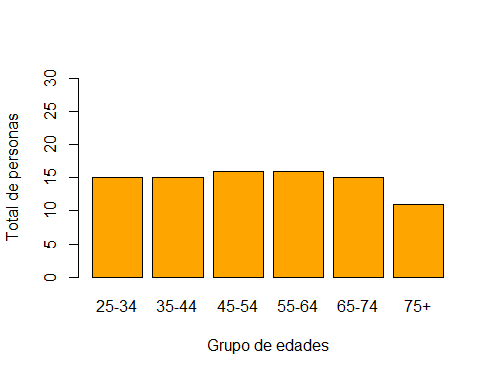
\includegraphics[scale = 0.7]{agegp.png}
	\caption{Gráfica de barra del grupos de edades} \label{fig:agegp}
\end{figure}
Los datos de los grupos de edades, se pueden observar en la Figura(\ref{fig:agegp}).

\begin{figure}
	\centering
	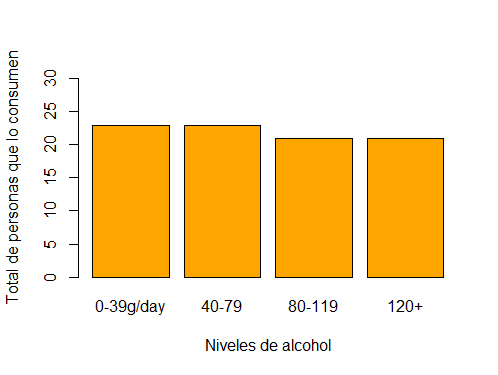
\includegraphics[scale = 0.7]{alcgp.png}
	\caption{Gráfica de barra sobre el consumo del alcohol} \label{fig:alcgp}
\end{figure}
Los datos del consumo de alcohol de las personas, se puede observar en la Figura(\ref{fig:alcgp}).

\begin{figure}
	\centering
	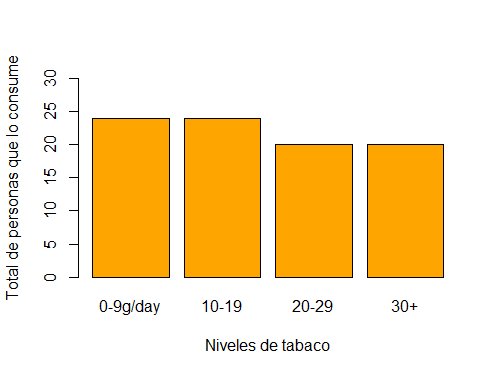
\includegraphics[scale = 0.7]{tobgp.png}
	\caption{Gráfica de barra sobre el consumo del tabaco} \label{fig:tobgp}
\end{figure}
Los datos del consumo de tabaco de las personas, se puede observar en la Figura(\ref{fig:tobgp}).

\begin{figure}
	\centering
	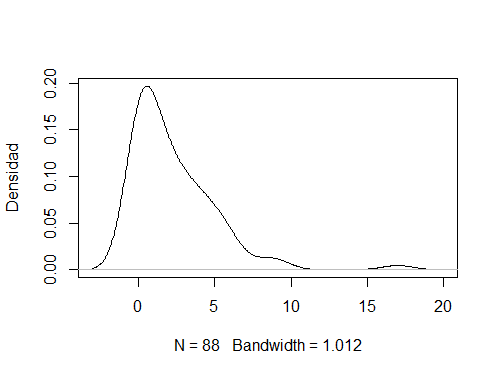
\includegraphics[scale = 0.7]{ncasos.png}
	\caption{Gráficas de densidad de los numeros de casos} \label{fig:ncasos}
\end{figure}
Los datos de numero de casos tiene un mínimo de 0.00 y un máximo de 17.00, media de 2.273 y mediana de 1.00. La Figura(\ref{fig:ncasos})se muestra la grafica de densidad de los numeros de casos.

\begin{figure}
	\centering
	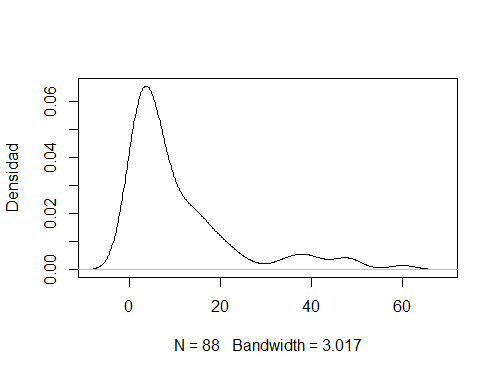
\includegraphics[scale = 0.7]{ncontr.png}
	\caption{Gráficas de densidad de los numeros controlados} \label{fig:ncontr}
\end{figure}
Los datos de los numeros controlados tiene un mínimo de 1.00 y un máximo de 60.00, media de 11.08 y mediana de 6.00. La Figura(\ref{fig:ncontr})se muestra la grafica de densidad de los numeros controlados.
\begin{figure}
	\centering
	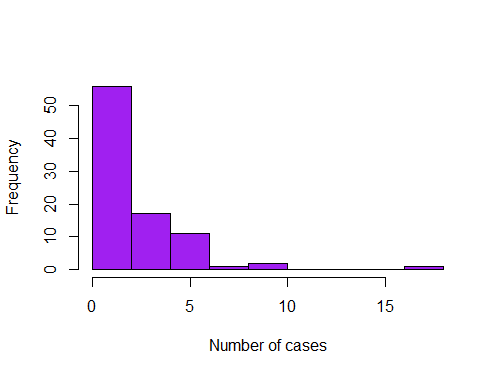
\includegraphics[scale = 0.7]{hist.png}
	\caption{Gráficas de densidad de los numeros controlados} \label{fig:hist}
\end{figure}

\begin{figure}
	\centering
	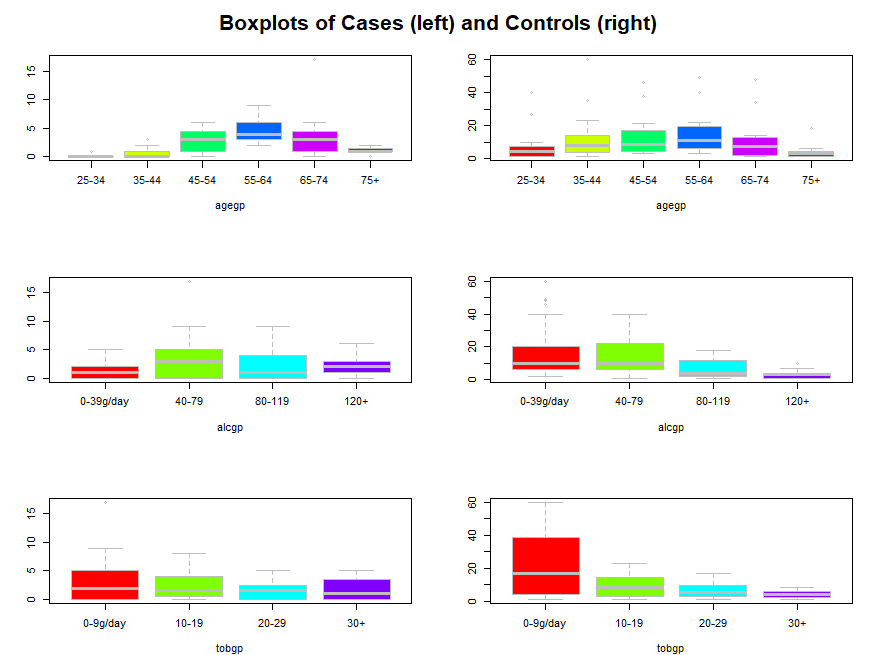
\includegraphics[scale = 0.65]{castrols1.png}
	\caption{Gráficas de densidad de los numeros controlados} \label{fig:castrols1}
\end{figure}
Agremamos un histograma en la que se puede ver la frecuencia de cada observacion y ademas se muestra la distribucion de las ocurrencias en cada categoria.La Figura(\ref{fig:hist}) se muestra la grafica, ademas de que tambien se realizo un bloxplots donde se puede ver los casos y controlados de cada categoria. La Figura(\ref{fig:castrols1}) se aprecia la grafica de bloxplots.\citep{repositorio}

\subsection{Estadística descriptiva de dos variables} \label{subsec:estadisticadescriptivados}

En las siguientes figuras (\ref{fig:scapl1}) y (\ref{fig:scapl2}) se muestran la relacion entre los casos y controles 
\begin{figure}
	\centering
	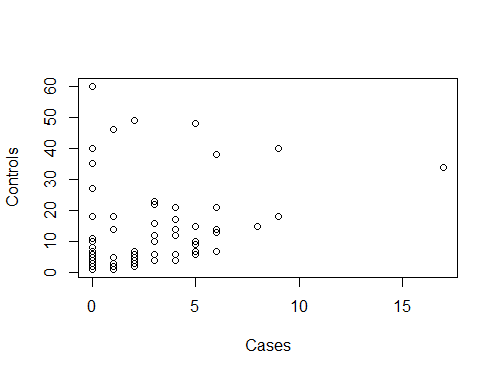
\includegraphics[scale = 0.65]{scapl1.png}
	\caption{Gráficas de densidad de los numeros controlados} \label{fig:scapl1}
\end{figure}
\begin{figure}
	\centering
	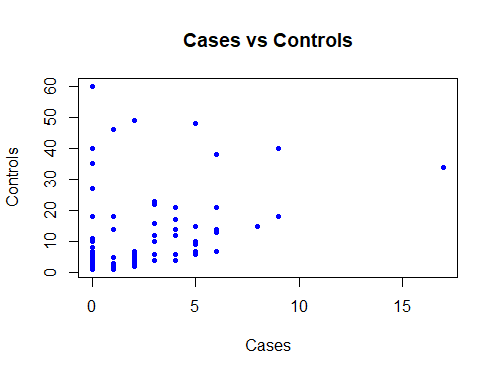
\includegraphics[scale = 0.65]{scalp2.png}
	\caption{Gráficas de densidad de los numeros controlados} \label{fig:scapl2}
\end{figure}

\bibliography{biblio}
\bibliographystyle{plainnat}

\end{document}